\documentclass[12pt,a4paper]{article}
\usepackage[T1]{fontenc}
\usepackage[utf8]{inputenc}
\usepackage[english]{babel}
\usepackage{mathptmx}
\usepackage[a4paper,margin=2.5cm,headheight=16pt]{geometry}
\usepackage{graphicx,caption,booktabs,tabularx,enumitem}
\usepackage{tikz}
\usetikzlibrary{arrows.meta,positioning,shapes.geometric}
\usepackage{xcolor}
\definecolor{baslik}{HTML}{17365D}
\usepackage{titlesec}
\titleformat{\section}{\Large\bfseries\color{baslik}}{\thesection}{.7em}{}
\titleformat{\subsection}{\large\bfseries\color{baslik}}{\thesubsection}{.7em}{}
\usepackage{fancyhdr,lastpage}
\pagestyle{fancy}
\fancyhf{}

\newcommand{\ogrenciad}{Full Name}
\newcommand{\ogrencino}{Student ID}

\fancyhead[L]{\small \ogrenciad\enspace--\enspace\ogrencino}
\fancyhead[R]{\small EHB326E}

\fancyfoot[C]{\thepage\ / \pageref{LastPage}}
\renewcommand{\headrulewidth}{0.4pt}
\usepackage{ragged2e}
\AtBeginDocument{\justifying}
\usepackage{hyperref}
\hypersetup{colorlinks=true,linkcolor=baslik,urlcolor=baslik,citecolor=baslik}

\newcommand{\raporbasligi}{Assignment Title}

\begin{document}
\begin{center}
{\Large\bfseries Istanbul Technical University}\\[5pt]
{\large EHB326E -- Assignment N Report}\\[18pt]
{\LARGE\bfseries\color{baslik}\raporbasligi}\\[15pt]
\ogrenciad\quad(\ogrencino)\\[5pt]
\today
\end{center}
\vspace{1em}

\section{Abstract}
Briefly describe the purpose of the design, the method used, and the verified results. Do not include unmeasured success or performance figures.

\section{Objective and Requirements}
State the objective and requirements of the assignment.

\section{Method and System Design}
If necessary, explain the system components and data flow. Adapt the diagram below to your own design.

\begin{figure}[htbp]\centering
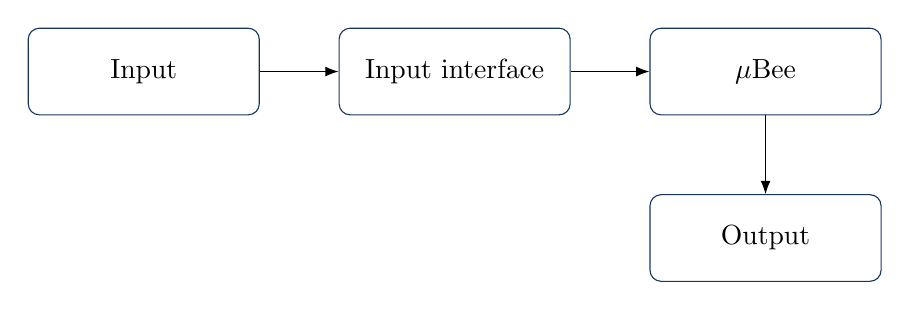
\begin{tikzpicture}[node distance=10mm and 10mm, >=Latex,
 block/.style={draw=baslik,rounded corners,align=center,minimum height=11mm,text width=27mm}]
\node[block] (girdi) {Input};
\node[block,right=of girdi] (arayuz) {Input interface};
\node[block,right=of arayuz] (sistem) {$\mu$Bee};
\node[block,below=of sistem] (cikti) {Output};
\draw[->] (girdi)--(arayuz);
\draw[->] (arayuz)--(sistem);
\draw[->] (sistem)--(cikti);
\end{tikzpicture}
\caption{Example system flow; update it to reflect the actual implementation.}
\label{fig:akis}
\end{figure}

\subsection{Implementation}
Do not paste code into the report. Explain the functions, inputs and outputs, timing, and design choices of the important modules; keep the source files separate in the submission package.

\section{Simulation and Findings}
Provide the test conditions, applied inputs (do not include code), expected behavior, and observed output. Refer to each figure in the text and interpret the results.

\begin{table}[htbp]\centering
\caption{Test and observation records}
\label{tab:test}
\begin{tabularx}{\linewidth}{@{}lXXX@{}}
\toprule
Test & Input / condition & Expected result & Observed result \\
\midrule
1 & [Fill in] & [Fill in] & [Fill in] \\
2 & [Fill in] & [Fill in] & [Fill in] \\
\bottomrule
\end{tabularx}
\end{table}

% Place the screenshot in the Images/ directory.
% Adjust cropping using trim={left bottom right top},clip.
% \begin{figure}[htbp]\centering
% \includegraphics[width=.9\linewidth,trim={12mm 8mm 12mm 8mm},clip]{Images/simulasyon.png}
% \caption{Simulation result and the corresponding test condition.}
% \label{fig:simulasyon}
% \end{figure}

\section{Verification and Evaluation}
Clearly state whether the design works correctly, which expected results were achieved, and any limitations. Support your evaluation with Table~\ref{tab:test}.

\section{Conclusion}
Briefly summarize the results obtained and the extent to which the design meets its objectives.

\begin{thebibliography}{99}
% Number the references used here in order; use \cite{ornek} in the text.
% \bibitem{ornek} Author/Institution, \emph{Title of the work or page}, year, \url{https://...}, accessed: DD.MM.YYYY.
\end{thebibliography}
\end{document}